%!TEX root = ../main.tex

The observed electrical resistance of copper is shown in \autoref{fig:copper}. The 
observed electrical resistances of niobium and silicon are displayed in \autoref{fig:niobium} and \autoref{fig:silicon} respectively. For an analysis of the gathered 
information refer to the following sections.

\begin{figure}
	\centering
	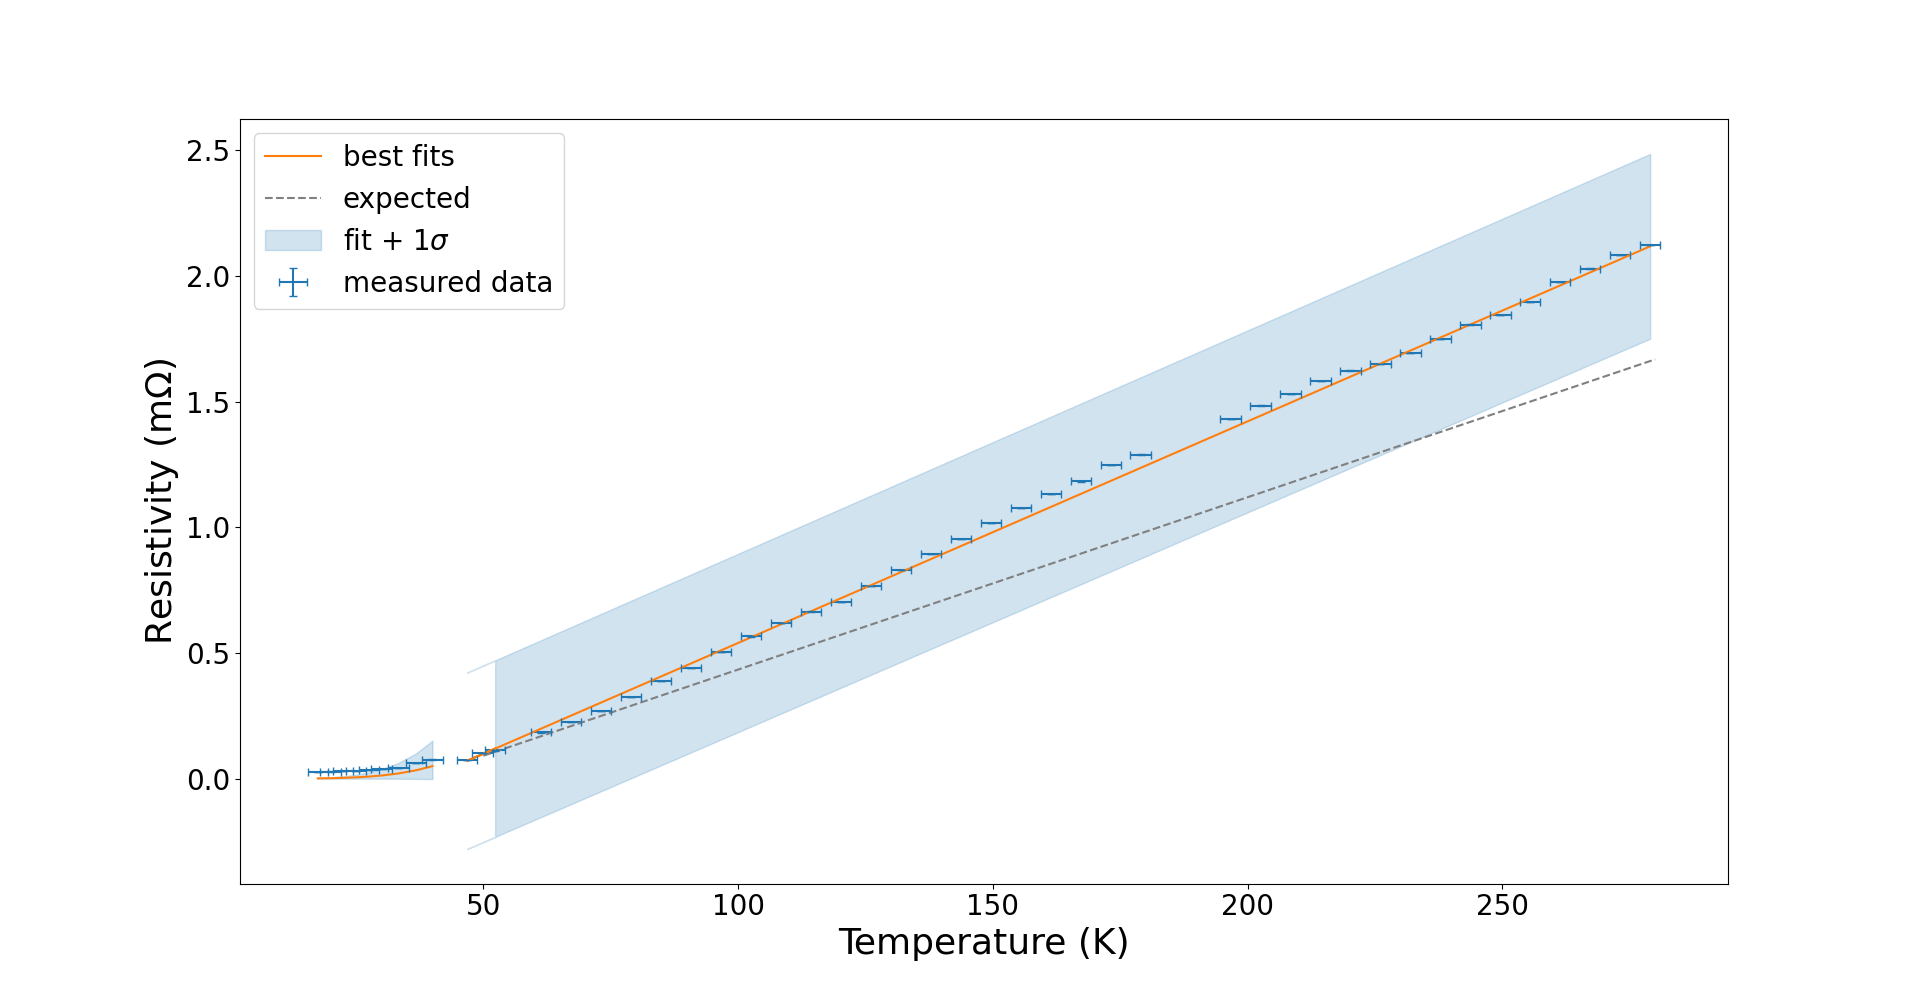
\includegraphics[width=1.0\textwidth]{./fig/copper.png}	
	\caption{Electrical resistance of copper at different temperatures}
	\label{fig:copper}
\end{figure}

\begin{figure}
	\centering
	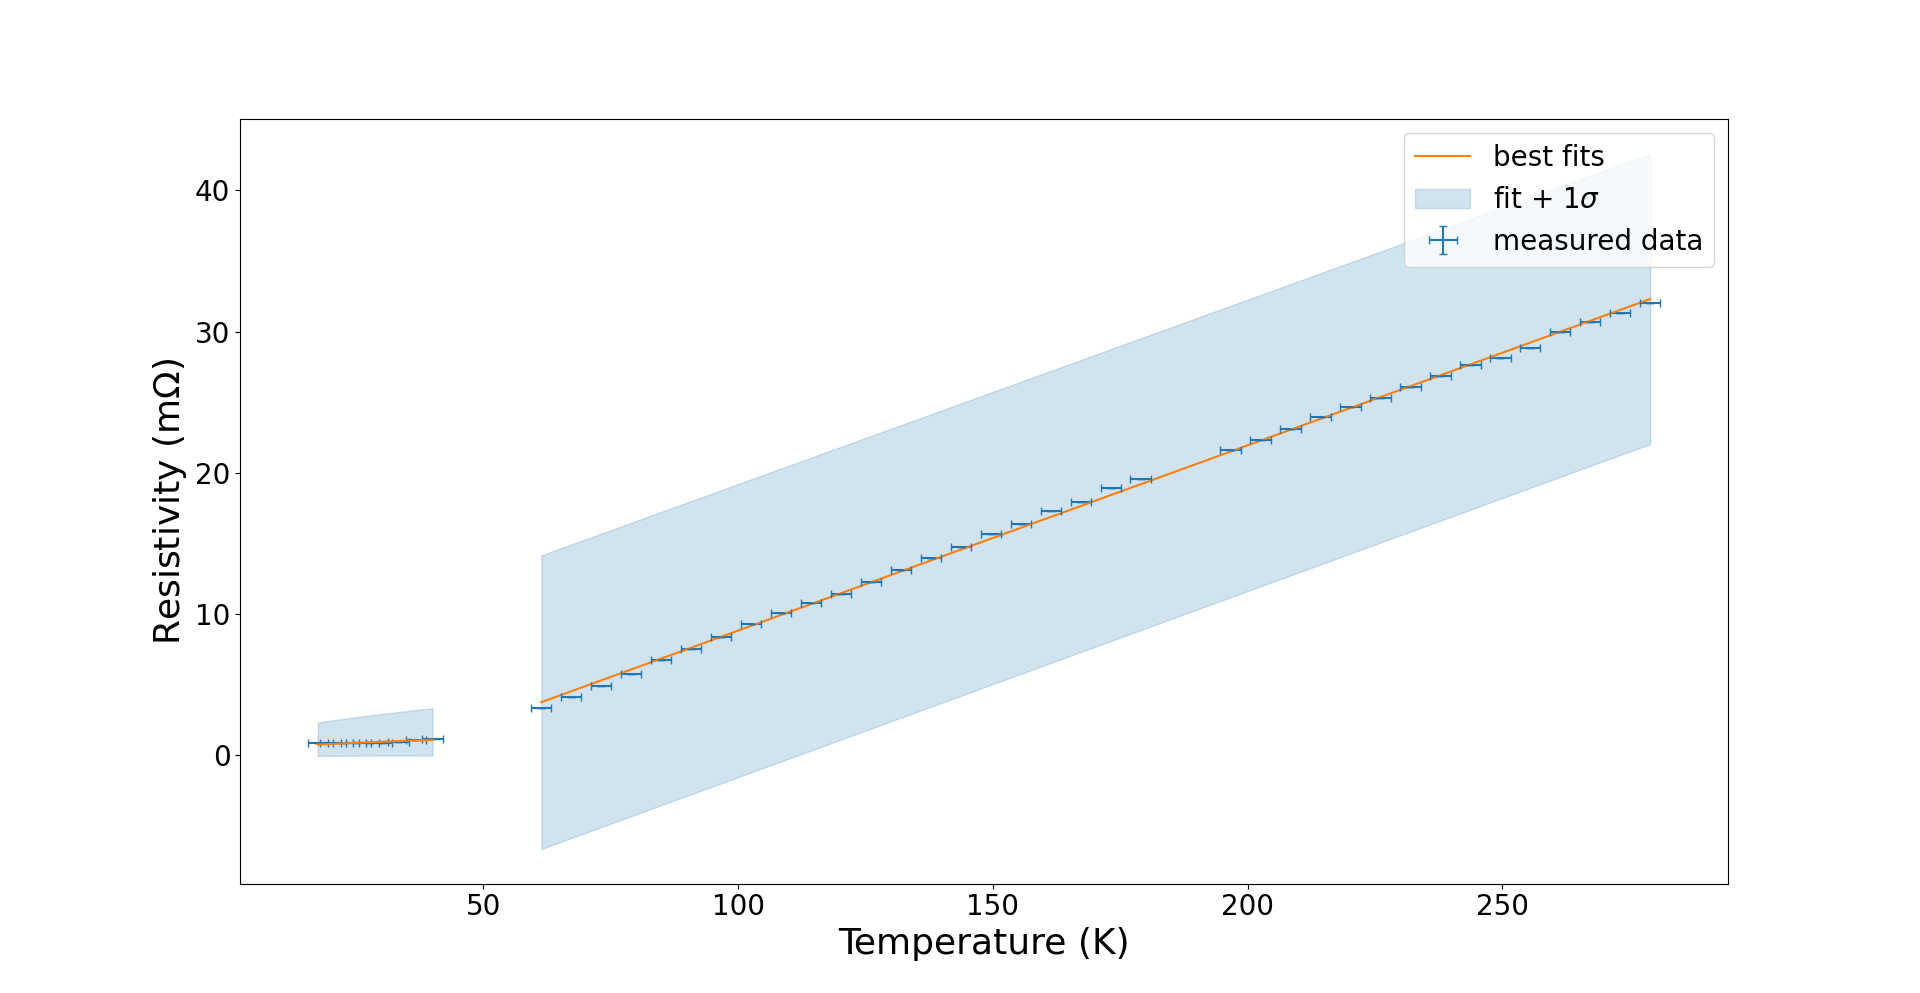
\includegraphics[width=1.0\textwidth]{./fig/niobium.png}
	\caption{Electrical resistance of niobium at different temperatures}
	\label{fig:niobium}
\end{figure}

\begin{figure}
	\centering
	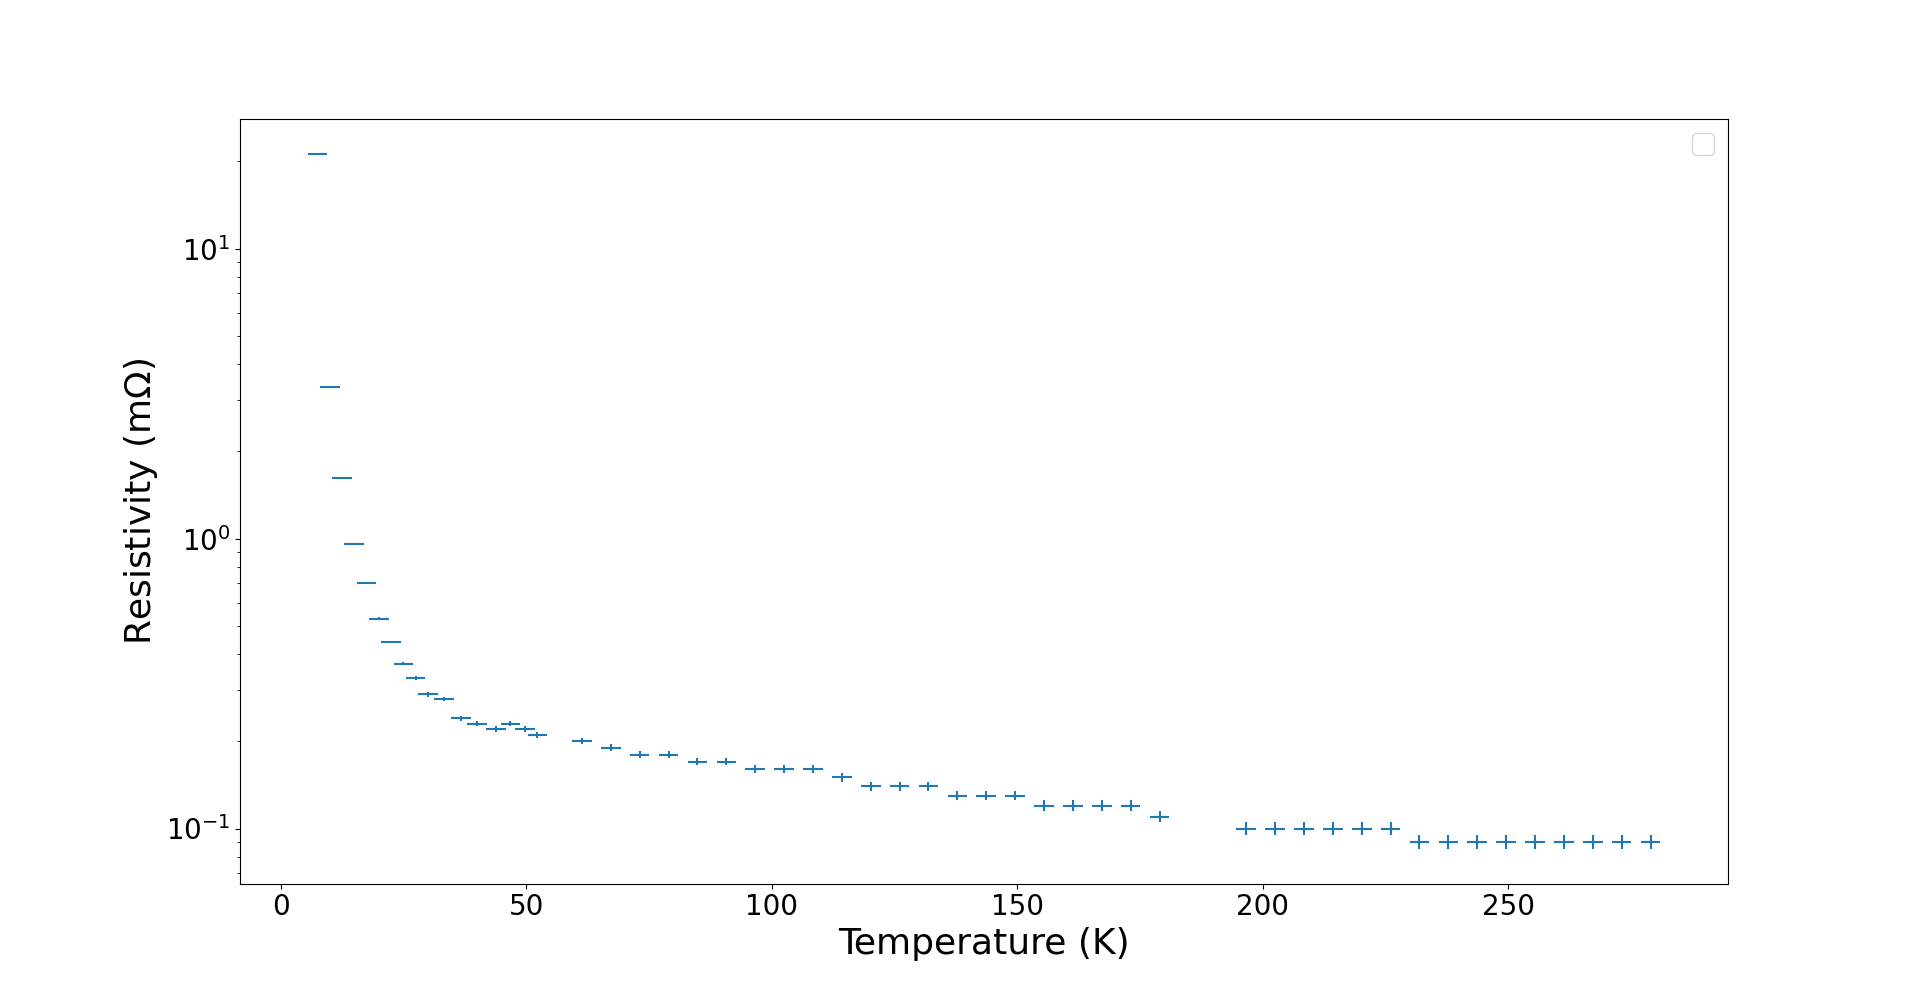
\includegraphics[width=1.0\textwidth]{./fig/silicon.png}
	\caption{Electrical resistance of silicon at different temperatures}
	\label{fig:silicon}
\end{figure}
